\documentclass[12pt,reqno,oneside]{article}
% \documentclass[12pt, final]{siamonline171218}
% \usepackage[pdfborder={0 0 0.5 [3 2]}]{hyperref}%
\usepackage[left=1in,right=1in,top=1in,bottom=1.25in]{geometry}%
\usepackage{amsmath}
\usepackage{amssymb}
\usepackage{amsthm}
\usepackage{graphicx}
\usepackage{enumerate}
\usepackage{float}
\usepackage{bm}
\usepackage[stable]{footmisc}

\usepackage{packages}
\usepackage{wrapfig}
\usepackage{subfigure}
\usepackage[font=footnotesize]{caption}

\newtheorem{theorem}{Theorem}
\newtheorem{lemma}[theorem]{Lemma}
\newtheorem{corollary}{Corollary}

\theoremstyle{definition}
\newtheorem{definition}[theorem]{Definition}

\theoremstyle{remark}
\newtheorem{remark}[theorem]{Remark}

\def\noi{\noindent}
\def\T{{\mathbb T}}
\def\R{{\mathbb R}}
\def\N{{\mathbb N}}
\def\Z{{\mathbb Z}}
\def\C{{\mathbb C}}
\def\Q{\mathbb{Q}}

\newcommand{\vK}{\bm{\mathit{K}}}
\newcommand{\calP}{\mathcal{P}}
\newcommand{\calA}{\mathcal{A}}

\setlength{\parindent}{0em}
\setlength{\parskip}{1em}
\renewcommand{\baselinestretch}{1.1}

\title{Research Statement}
\date{\vspace{-12ex}}

\begin{document}

\thispagestyle{empty}

\maketitle

My main research interest is in nonlinear waves and coherent structures. Examples of coherent structures include solitary waves, which are localized disturbances that maintain their shape as they propagate through a medium at a constant velocity, and breathers, which are localized, oscillatory patterns. In particular, I am interested in applications to nonlinear optics and pattern formation on lattices and networks.

\section{Multi-pulse solitary waves}

Solitary waves were originally discovered as a water wave phenomenon, but they have applications in diverse fields such as fiber optics, plasma physics, and quantum mechanics; they can also be used for models in biology and neuroscience. More generally, many nonlinear, dispersive PDEs have solitary wave solutions. In particular, I study the existence and stability of multi-pulse solitary waves in Hamiltonian systems. Multi-pulses are disturbances which resemble multiple, well separated copies of a single solitary wave. In addition to having applications to fields such as nonlinear optics and neuroscience \cite{Evans1982}, multi-pulses are interesting mathematically. Since a multi-pulse structure maintains its shape as it is transmitted, it may appear at first glance that the individual pulses do not interact. The underlying dynamics, however, is inherently nonlinear, and the interaction between the pulses is revealed when we perturb the structure. I am interested in how the spectral properties of these multi-pulses can explain how they react to perturbations.

\subsection{Mathematical approach}

My primary mathematical approach comes from spatial dynamics. From this viewpoint, a solitary wave is a homoclinic orbit evolving in the spatial variable. This primary homoclinic orbit is an intersection of the stable and unstable manifolds of an equilibrium point, which represents the rest state of the system. Some spectral properties, such as the essential spectrum, only depend on the rest state. Multi-pulses are multi-loop homoclinic orbits, which can be constructed using Lin's method \cite{Lin2008}, a version of the Lyapunov-Schmidt method used to find solutions which remain near a homoclinic orbit. Heuristically, this process involves gluing together multiple copies of the primary homoclinic orbit. I also use Lin's method to construct periodic orbits and multi-loop periodic orbits. To find eigenvalues associated with multi-pulses, I use two main tools. First, I use Lin's method as in \cite{Sandstede1998} to construct eigenfunctions as perturbations of the eigenfunctions associated with the primary solitary wave. I also use the Krein matrix \cite{Kapitula2013a,Kapitula2020}, which is a projection of an eigenvalue problem onto a finite dimensional subspace.

In addition to theoretical work, I also use numerical analysis, both to generate hypotheses and to verify theoretical results. For multi-pulses, I start by constructing the primary solitary wave, which either involves parameter continuation from a known solution using the software package AUTO or an energy minimization method such as the string method \cite{Chamard2011} or the mountain pass method \cite{Chen1997}. I then glue together multiple copies of the primary solitary wave and use a Newton solver such as Matlab's \texttt{fsolve} function or a conjugate gradient method to construct a multi-pulse. For the spectrum, I first discretize the problem, usually with a Fourier or polynomial spectral method. I then find the spectrum using a numerical eigenvalue solver. I also use AUTO to study how eigenvalues change as parameters are varied.

I work with the following four Hamiltonian equations in my research:
\begin{align*}
\partial_t u - \partial_x^5 u + \partial_x^3 u + 2 u \partial_x u &= 0 && \text{fifth-order Korteweg de-Vries equation} \\
\partial_t^2 u + \partial_x^4 u + \mathrm{e}^{u-1} - 1 &= 0 &&\text{Chen-McKenna suspension bridge equation} \\
i u_t + \frac{\beta_4}{24}u_{xxxx} - \frac{\beta_2}{2}u_{xx} + \gamma |u|^2 u &= 0 && 
\text{fourth-order nonlinear Schr{\"o}dinger equation } \\
i\partial_t u_n + d(u_{n+1} - 2 u_n + u_{n-1}) + |u_n|^2 u_n &= 0 &&\text{discrete nonlinear Schr{\"o}dinger equation}
\end{align*}
The fifth-order Korteweg de-Vries equation (KdV5) is a weakly nonlinear long wave approximation to capillary-gravity wave problem which also has applications to plasma physics and laser optics \cite{Pelinovsky2007}. The Chen-McKenna suspension bridge equation is a smooth approximation to a model for waves propagating on an infinitely long suspended beam, and is motivated by observations of traveling waves on suspension bridges \cite{McKenna1990,Chen1997}. The fourth-order nonlinear Schr{\"o}dinger equation (NLS4) is a variant of the nonlinear Schr{\"o}dinger equation (NLS) which was introduced to account for the role of small fourth-order dispersion terms in the propagation of intense laser beams in a bulk medium with Kerr nonlinearity \cite{Karpman2000,Tam2020}. The discrete nonlinear Schr{\"o}dinger equation (DNLS) is the discrete analogue to the nonlinear Schr{\"o}dinger equation and has applications to nonlinear optics and condensed matter physics \cite{Kevrekidis2009}. KdV5 and Chen-McKenna have traveling wave solutions of the form $u(x, t) = \phi(x - ct)$, where $c$ is the wavespeed. NLS4 and DNLS have rotating waves of the form $u = e^{i\omega t}\phi$, where $\omega$ is the rotational frequency. All four equations have primary solitary wave solutions \cite{Pelinovsky2007,Berg2018,Parker2020NLS4,Kevrekidis2009}. For appropriate values of the parameters $c$ and $\omega$, they also have multi-pulse solutions \cite{Buffoni1996,SandstedeStrut,Parker2020NLS4,Parker2020}.

\subsection{Interaction eigenvalues of multi-pulses}

The main focus of my research involves determining the spectrum associated with the linearization about a multi-pulse solution. In general, each pulse that is added to a multi-pulse structure is associated with one or more eigenvalues in the spectrum. I refer to these as interaction eigenvalues, since they result from nonlinear interactions between neighboring pulses. For a large class of systems, this problem is solved in \cite{Sandstede1998}, which reduces the problem of to finding the eigenvalues of a matrix.

\begin{wrapfigure}[8]{R}{6cm}
\includegraphics[width=6cm]{images/inteigpattern.eps}
\caption{Possible interaction eigenvalue patterns.} 
\label{fig:inteigpattern}
\end{wrapfigure}
The systems I study are Hamiltonian, which are not covered by the results of \cite{Sandstede1998}. On one hand, the Hamiltonian structure is very helpful, since all eigenvalues must come in quartets of the form $\pm \alpha \pm \beta i$. This means that each additional set of interaction eigenvalues must come in one of the three patterns in \cref{fig:inteigpattern}. On the other hand, the presence of any eigenvalue with nonzero real part implies that there is an unstable eigenvalue. This means that Hamiltonian systems cannot be dissipative, which makes stability analysis more difficult. 

My main results relate the spectral pattern of the interaction eigenvalues to the underlying geometry of the multi-pulse. In all cases, the spectral pattern is determined by the geometry of the underlying multi-pulse solution. For the continuous systems (KdV5, Chen-McKenna, and NLS4), multi-pulses exist in discrete families. The distances between neighboring pulses are constrained to be an integer multiple of a phase parameter. This constraint is a consequence of the specific alignment of manifolds necessary for multi-pulses to occur, and these integers represent the number of twists made by the stable and unstable manifolds near the equilibrium at 0. An $m-$pulse, therefore, can be described by $m-1$ nonnegative integers $\{ k_1, \dots, k_{m-1} \}$. For KdV5 \cite{Pelinovsky2007} and Chen-McKenna \cite{Kapitula2020}, the eigenvalue pattern is determined by whether these integers are even or odd. For DNLS, a multi-pulse is constructed from single pulses which can either be in phase or out of phase, and the eigenvalue pattern is determined by these phase differences. See \cref{fig:eigpatterns} for examples of these patterns. For NLS4, all multi-pulses are unstable since there is always an interaction eigenvalue with positive real part \cite{Parker2020NLS4}. 

\begin{figure}
\centering
\begin{tabular}{ccc}
\includegraphics[width=4cm]{images/dp1.eps} &
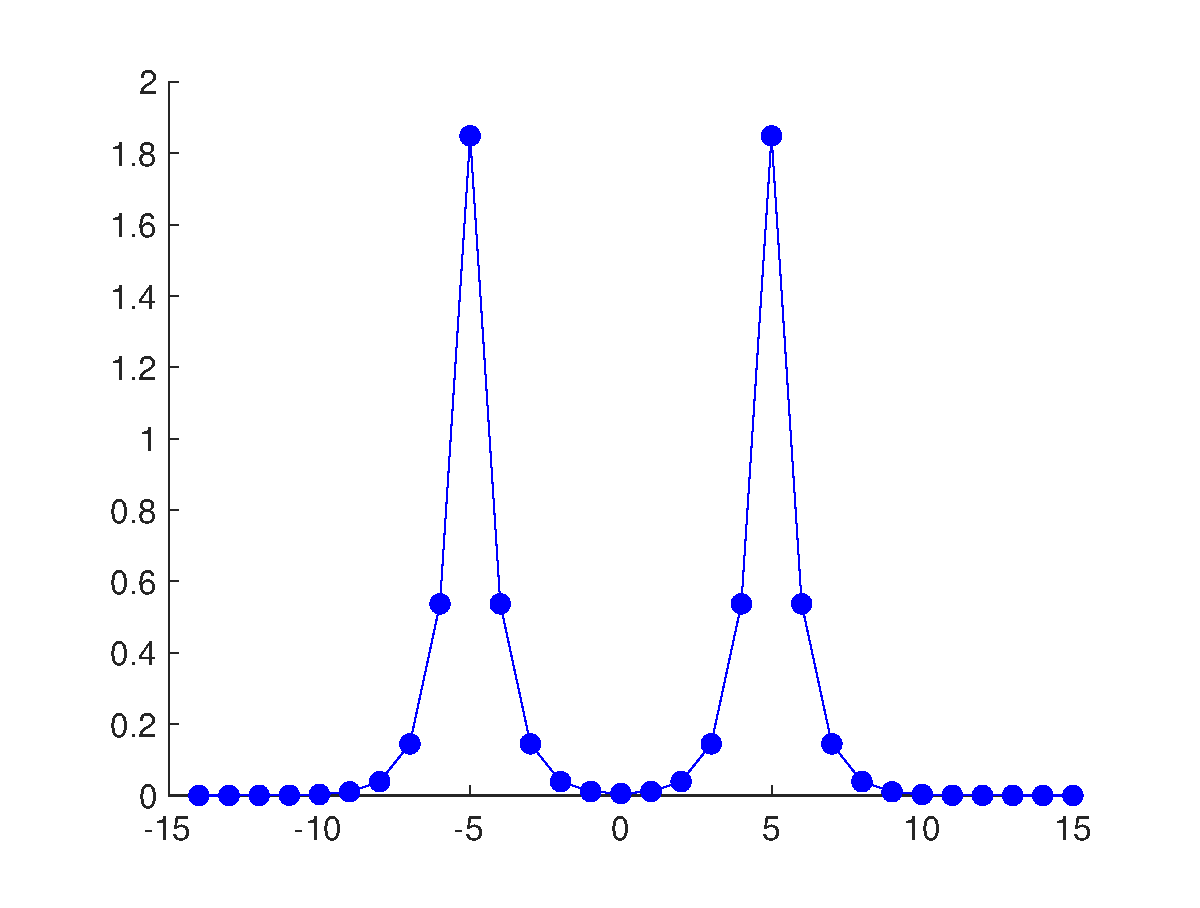
\includegraphics[width=4cm]{images/dnls2unstable.eps} &
\includegraphics[width=4cm]{images/unstableeigpattern.eps} \\
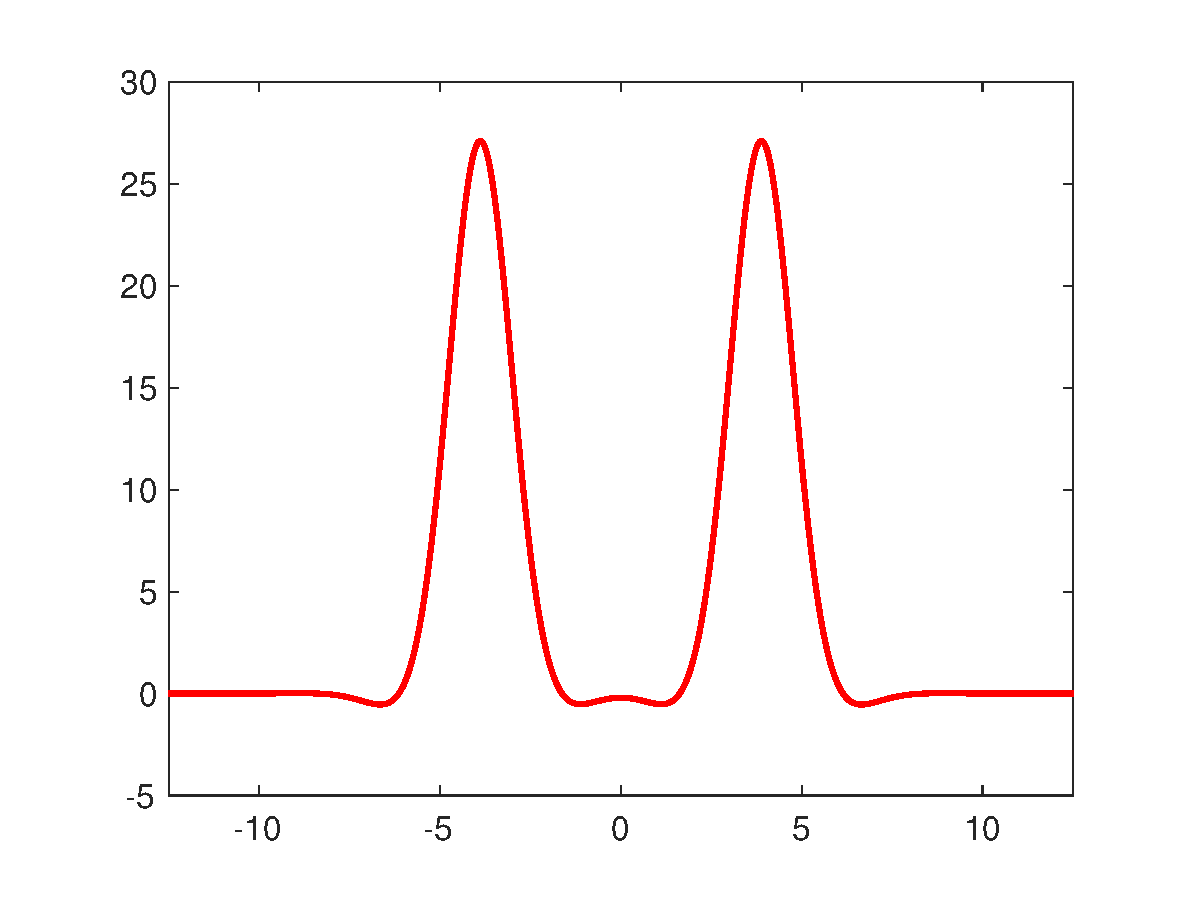
\includegraphics[width=4cm]{images/dp2.eps} &
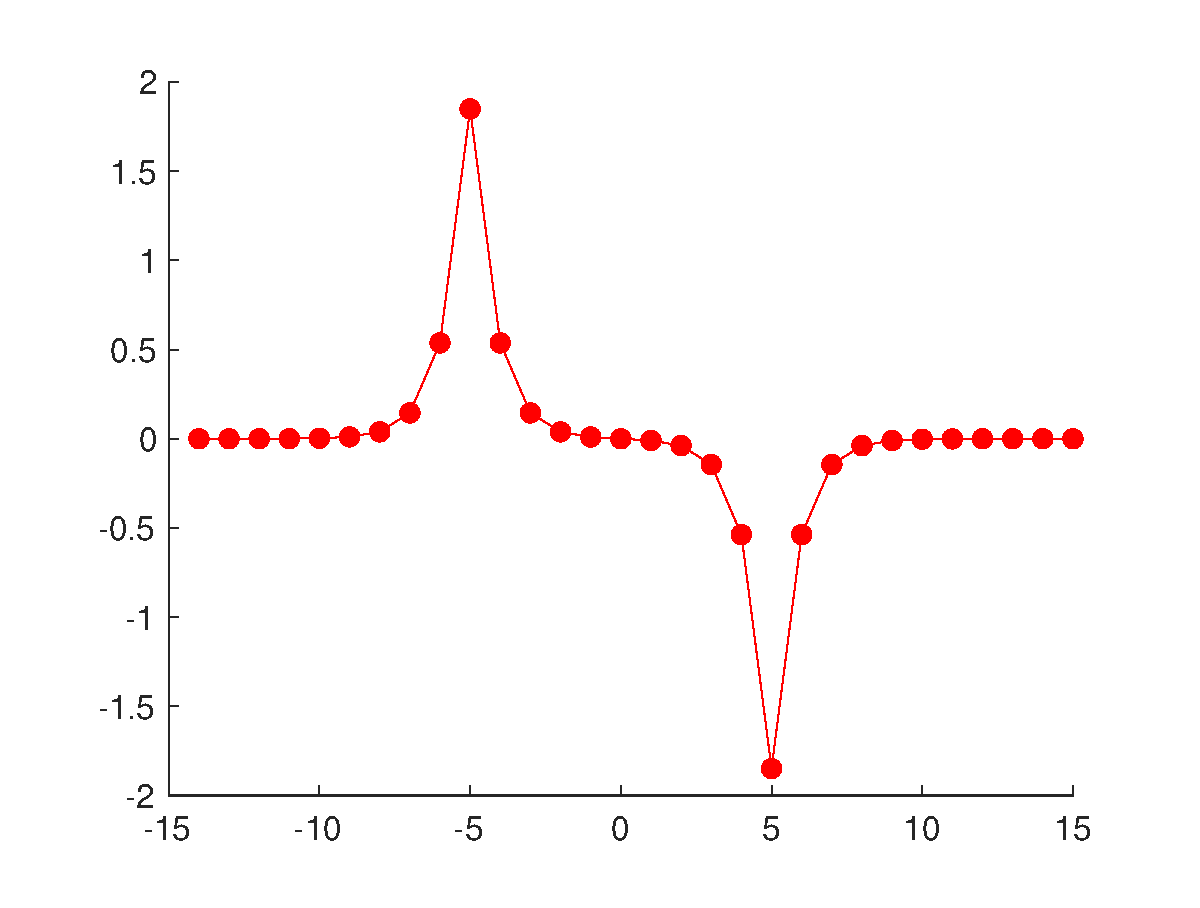
\includegraphics[width=4cm]{images/dnls2stable.eps} &
\includegraphics[width=4cm]{images/stableeigpattern.eps} 
\end{tabular}
\caption{Double pulses for KdV5 (left) and DNLS (center). Corresponding eigenvalue pattern (right).}
\label{fig:eigpatterns}
\end{figure}

For Chen-McKenna, I have proved these results analytically in \cite{Kapitula2020} using an extension of the Krein matrix. For DNLS, I use Lin's method to extend the stability results of \cite{Kapitula2001,Kapitula2001a} to solutions away from the anti-continuum limit \cite{Parker2020}. For NLS4, I adapt the extension of Lin's method for systems with two continuous symmetries in \cite{Manukian} to Hamiltonian systems in \cite{Parker2020NLS4}. For KdV5, the analysis is complicated by the essential spectrum, which is the entire imaginary axis. Any purely imaginary interaction eigenvalues would be embedded in the essential spectrum. Using an exponentially weighted space, I am able to prove an instability criterion for multi-pulses. For the cases where numerical analysis suggests that there are purely imaginary interaction eigenvalues, I can only prove that they are purely imaginary to leading order. To circumvent this problem, I look at periodic multi-pulse solutions.

\subsection{Periodic multi-pulses}

\begin{figure}[H]
\begin{center}
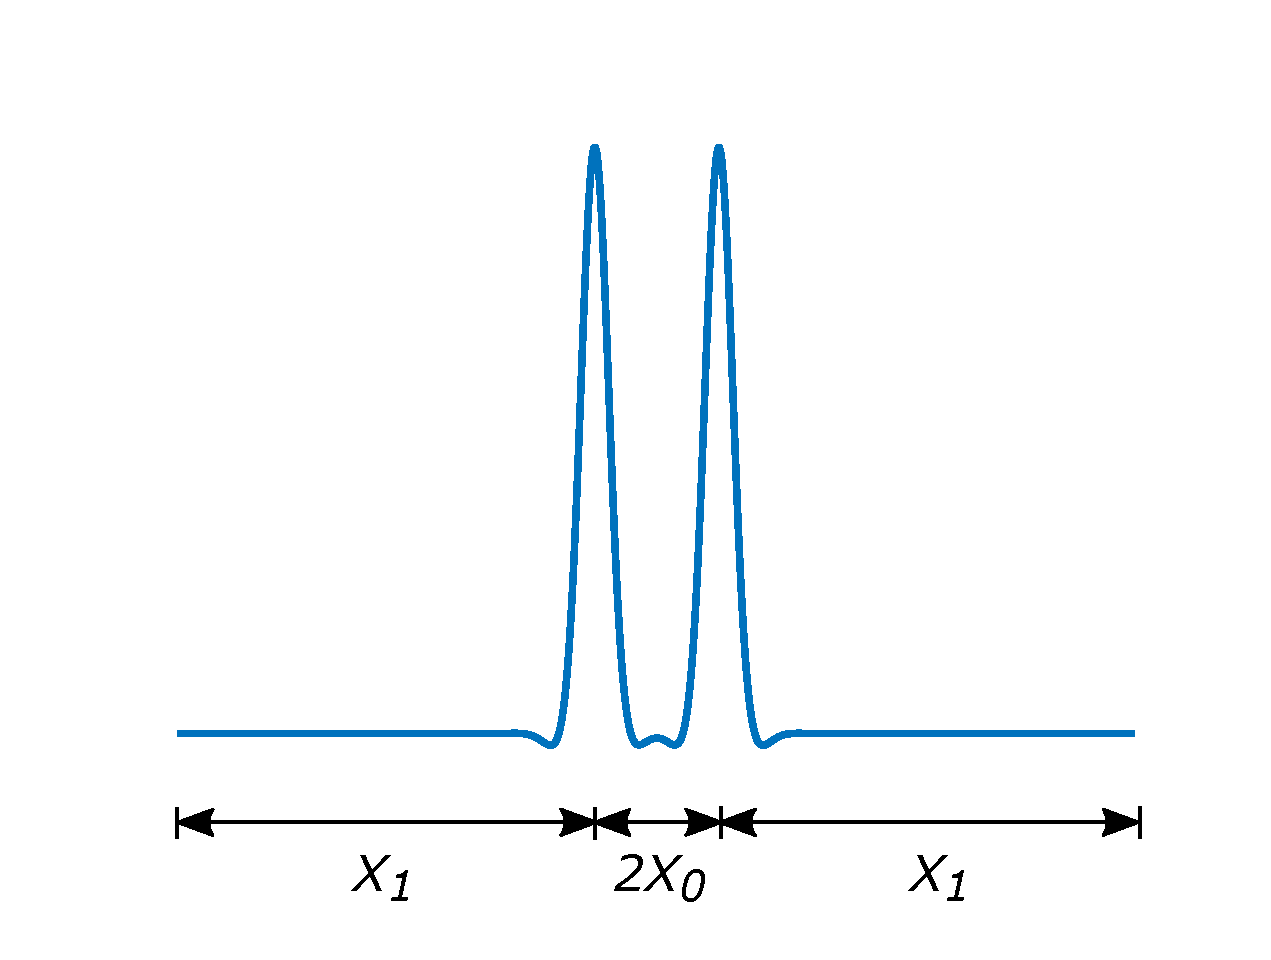
\includegraphics[width=8cm]{images/DPperiodic.eps} \hspace{-1cm}
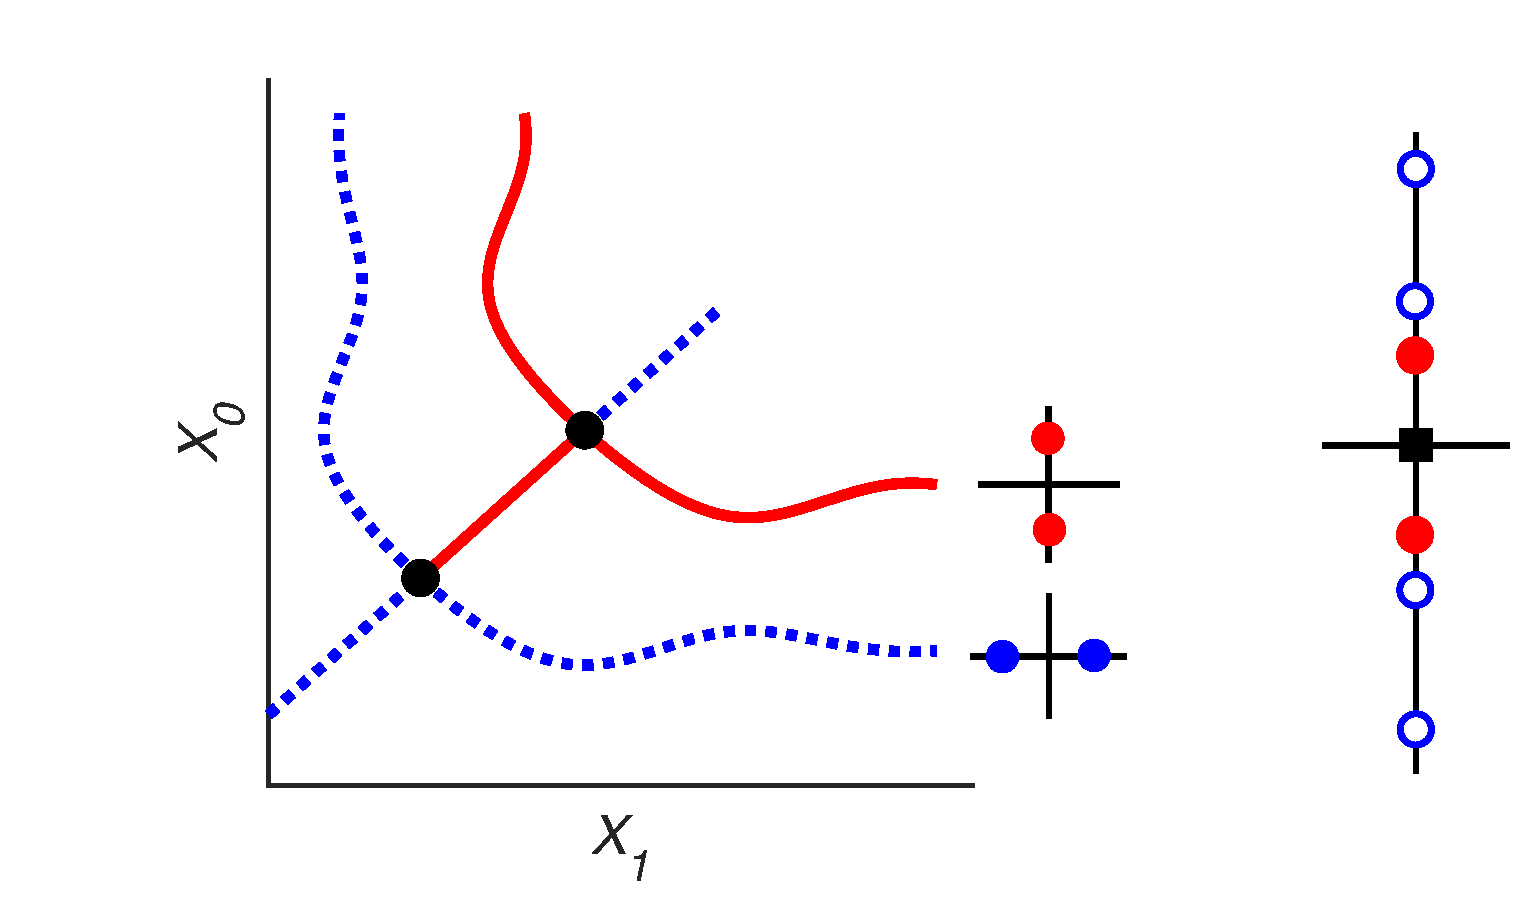
\includegraphics[width=9cm]{images/2pitchforkcoloreig2.eps}
\end{center}
\caption{Construction, bifurcation, and spectrum of periodic 2-pulses for KdV5.}
\label{fig:periodic}
\end{figure}

A periodic multi-pulse is a periodic orbit which contains multiple peaks. From a spatial dynamics perspective, these are multi-loop periodic orbits which are close to the primary homoclinic orbit. A periodic 2-pulse is constructed by gluing two single pulses together at both ends. Since this construction involves two length parameters $X_0$ and $X_1$ (see \cref{fig:periodic}, left), there is an extra degree of freedom when compared to the 2-pulses on the real line. As a consequence, there is a continuous family of periodic 2-pulses, in which asymmetric periodic 2-pulses ($X_0 \neq X_1$) bifurcate from symmetric periodic 2-pulses ($X_0 = X_1$) a series of pitchfork bifurcations (\cref{fig:periodic}, center) \cite{ParkerKdV}. The advantage of looking at periodic solutions is that the essential spectrum becomes a discrete set of purely imaginary eigenvalues (blue open circles in \cref{fig:periodic}, right). Purely imaginary interaction eigenvalues can then lie in gaps between essential spectrum eigenvalues, which avoids the problem of embedded eigenvalues. 

The eigenvalues associated with a periodic multi-pulse can be found by solving a block matrix equation \cite[Theorem 5.3]{ParkerKdV} which, to leading order, is given by
\begin{equation}\label{blockmatrix}
\det \begin{pmatrix}
K(\lambda) - \frac{1}{2} \lambda \tilde{M} K^+(\lambda) & \lambda^2 M_c I \\
-\frac{1}{2} \lambda M_c K^+(\lambda) & A - \lambda^2 MI  
\end{pmatrix} = 0
\end{equation}
The essential spectrum eigenvalues are encoded by the matrix $K(\lambda)$, which, to leading order, only depends on the background state and the periodic domain $[-X, X]$, where $X = X_0 + X_1$. The interaction eigenvalues are encoded by the matrix $A$, which depends on the geometry of the multi-pulse. As long as $X$ is not too large, the interaction eigenvalues and essential spectrum eigenvalues do not interfere with each other. For a periodic 2-pulse, there is a pair of interaction eigenvalues which is either real or purely imaginary depending on the geometry of the periodic 2-pulse (\cref{fig:periodic}, center); the eigenvalue pattern switches between real and imaginary at the pitchfork bifurcation points.  

There is an additional complication in the periodic case. It is possible to increase $X$ so that an essential spectrum eigenvalue becomes close to an interaction eigenvalue. At a critical value of $X$, there is a collision between one of the essential spectrum eigenvalues and a purely imaginary interaction eigenvalue. As $X$ is further increased, I prove that a brief instability bubble is formed, wherein the two eigenvalues collide, move off the imaginary axis, trace an approximate circle in the complex plane, and recombine on the imaginary axis in a ``reverse''  collision (see \cref{fig:kreinbubble1} for a cartoon) \cite{ParkerKdV}. This instability bubble, which we call a Krein bubble, is a direct consequence of the block matrix reduction \cref{blockmatrix}. A numerical simulation of the Krein bubble, performed using parameter continuation with AUTO, is shown in \cref{fig:kreinbubble1} (right). The location and size of the Krein bubble in the simulation agree with that predicted by the theory \cite{ParkerKdV}.

Future work includes running time-stepping simulations for 2-periodic pulses in these Krein bubbles to see what type of instability they cause. In addition, it would be interesting to explore if these Krein bubbles occur for more complex multi-pulse structures, such as triple pulses, and if they occur in other systems.

\begin{figure}[H]
\begin{center}
\begin{tabular}{c}
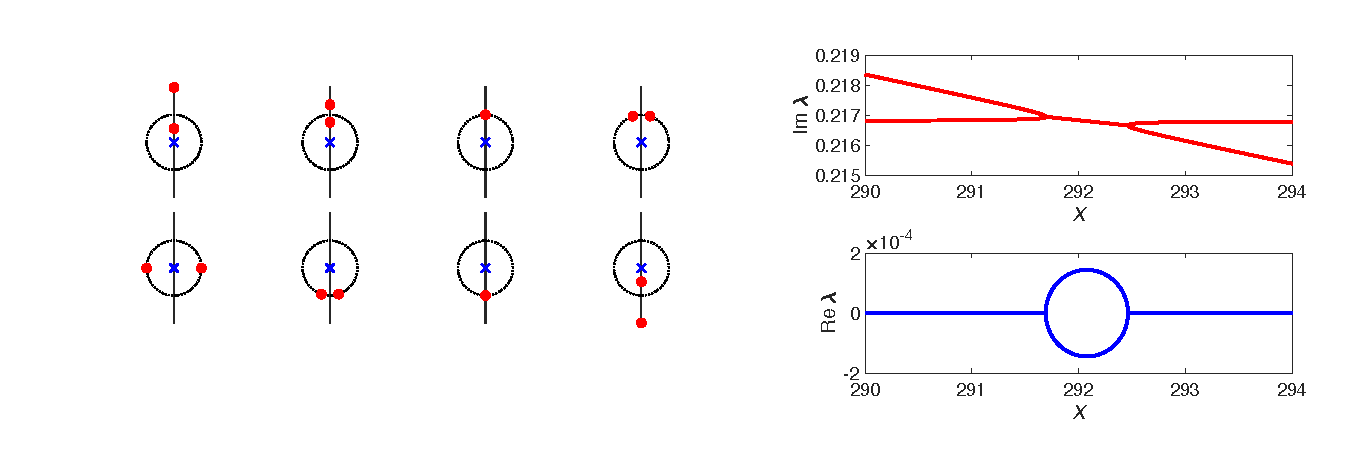
\includegraphics[width=0.9\textwidth]{images/KreinBubbleBoth}
\end{tabular}
\end{center}
\caption{Krein instability bubble cartoon (left) and numerical simulation for KdV5 (right).}
\label{fig:kreinbubble1}
\end{figure}

\subsection{Stability of multi-pulses}

How is the interaction eigenvalue pattern related to the stability of multi-pulse structures? I study this for KdV5 using numerical time-stepping, beginning with initial conditions with are close to multi-pulse solutions. At each time point, I compute the distance between the two pulses and its derivative, which I call the pulse relative velocity. I then plot trajectories of this reduced, two-dimensional system (\cref{fig:KdV5timestep}, left panel). 
\begin{figure}[H]
\begin{center}
\begin{tabular}{cc}
\includegraphics[width=7cm]{images/phaseportrait}  &
\includegraphics[width=7cm]{images/simplephaseportrait}
\end{tabular}
\end{center}
\caption{Phase portrait for peak relative velocity vs. peak distance for time-stepping of KdV5 with initial conditions near the first four double pulses (left panel). Phase portrait of \cref{harmonicvary} (right panel).
}
\label{fig:KdV5timestep}
\end{figure}
For 2-pulse solutions to KdV5, there are two alternating eigenvalue patterns: unstable (pair of real interaction eigenvalues) and neutrally stable (pair of imaginary interaction eigenvalues). The unstable pattern corresponds to a saddle node; a perturbation near this equilibrium will cause the two pulses to repel each other (\cref{fig:KdV5timestep}, left). The stable pattern corresponds to a center; a perturbation near this equilibrium will cause the two pulses to oscillate about their center of mass (\cref{fig:KdV5timestep}, right). 
\begin{figure}[H]
\begin{center}
\begin{tabular}{cc}
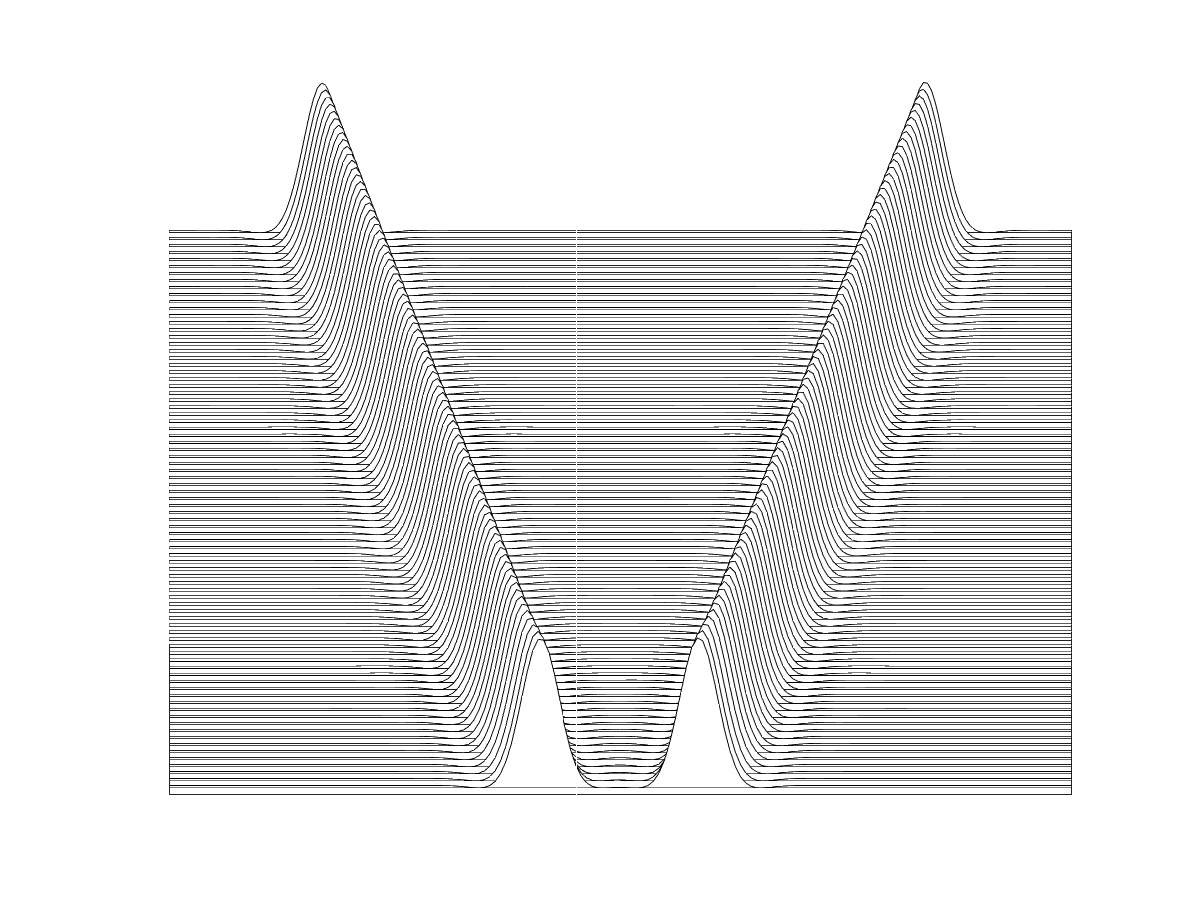
\includegraphics[width=7cm]{images/waterfallunstable.eps}  &
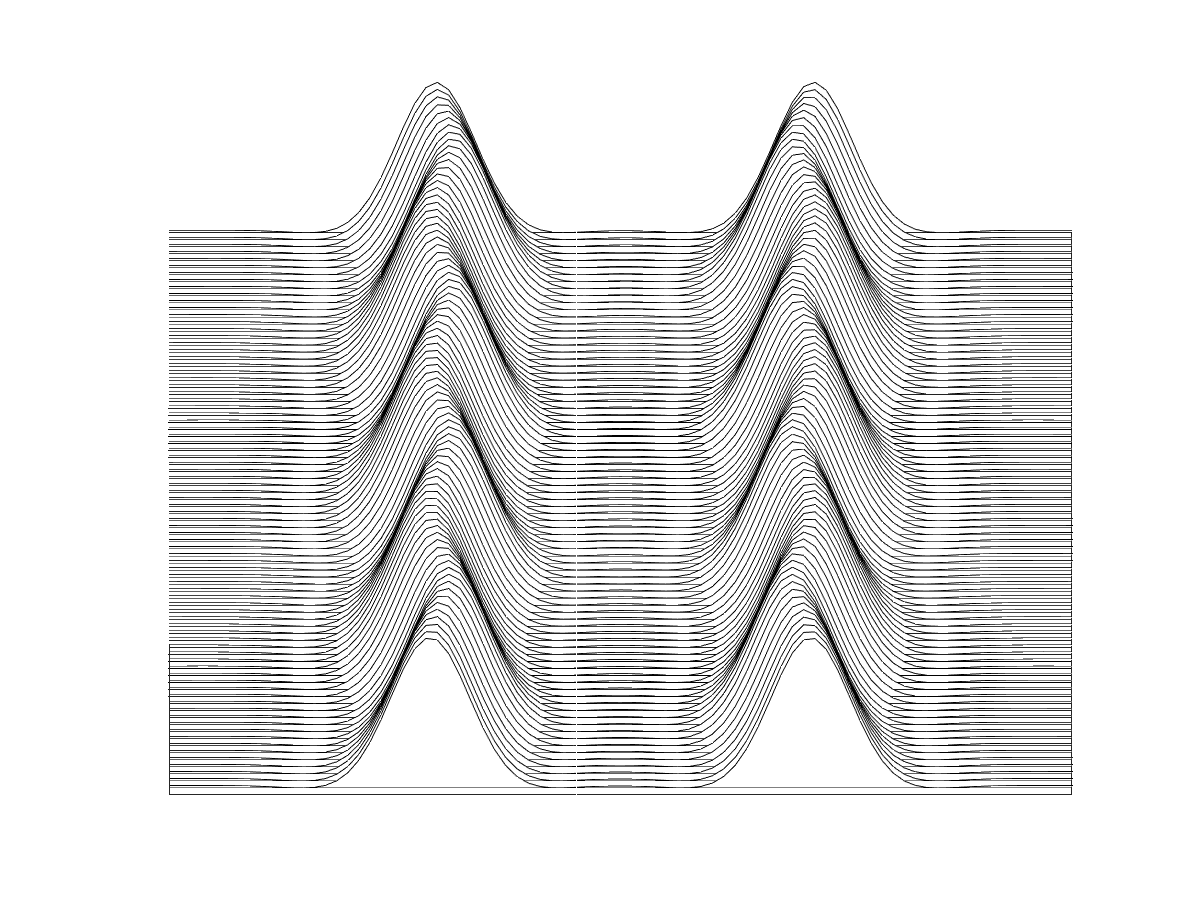
\includegraphics[width=7cm]{images/waterfallstable.eps}
\end{tabular}
\end{center}
\caption{Timestepping simulation for perturbation of unstable (left) and stable (right) double pulses for KdV5.}
\label{fig:KdV5timestep}
\end{figure}
The phase portrait resembles that of the planar system \eqref{harmonicvary}, which is a harmonic oscillator with spatially varying restoring force (\cref{fig:KdV5timestep}, right panel).
\begin{equation}\label{harmonicvary}
\begin{aligned}
\dot{x} &= y \\
\dot{y} &= C e^{-\alpha_0 x} \sin \beta_0 x
\end{aligned}
\end{equation} 

\section{Twisted multi-core optical fibers}

There has been much recent interest in the propagation dynamics of light pulses through multi-core optical fibers. In particular, optical transmission properties can be tuned by introducing a twist to the individual fibers in the bundle. A simple example is a circular multi-core fiber \cite{Longhi2016,CastroCastro2016,Parto2017} (\cref{fig:twist}).
\begin{figure}[H]
\begin{center}
\begin{tabular}{cc}
\includegraphics[width=6.5cm]{images/twist2.png} &
\includegraphics[width=4cm]{images/twistmulticore.png}
\end{tabular}
\end{center}
\caption{Schematic of circular multi-core fiber \cite{Longhi2016} (left) and twisted multi-core fiber with eight waveguides \cite{Parto2017} (right).}
\label{fig:twist}
\end{figure}
The propagation of light through this system can be described by the coupled mode equations
\begin{equation*}
i \partial_z c_n = k \left(e^{-i\phi}c_{n+1} + e^{i\phi}c_{n-1}\right) + |c_n|^2 c_n,
\end{equation*}
for $n = 1, \dots, N$, where $c_0 = c_{N}$ and $c_{N+1} = c_1$ due to the circular geometry, $k$ is the strength of the nearest-neighbor coupling, and $\phi$ is a parameter representing the twist of the fibers. Standing wave solutions of the form $c_n = a_n e^{i (\omega z + \theta_n) }$ exist, and, in particular, standing waves where the energy is concentrated at a single site are stable. When the twist parameter and the number of fibers in the bundle are related by $\phi = \pi/N$, the stable standing wave solution has a ``dark node'' with no optical activity opposite the node of maximum intensity \cref{fig:twistcn}. 
\begin{figure}[H]
\begin{center}
\begin{tabular}{c}
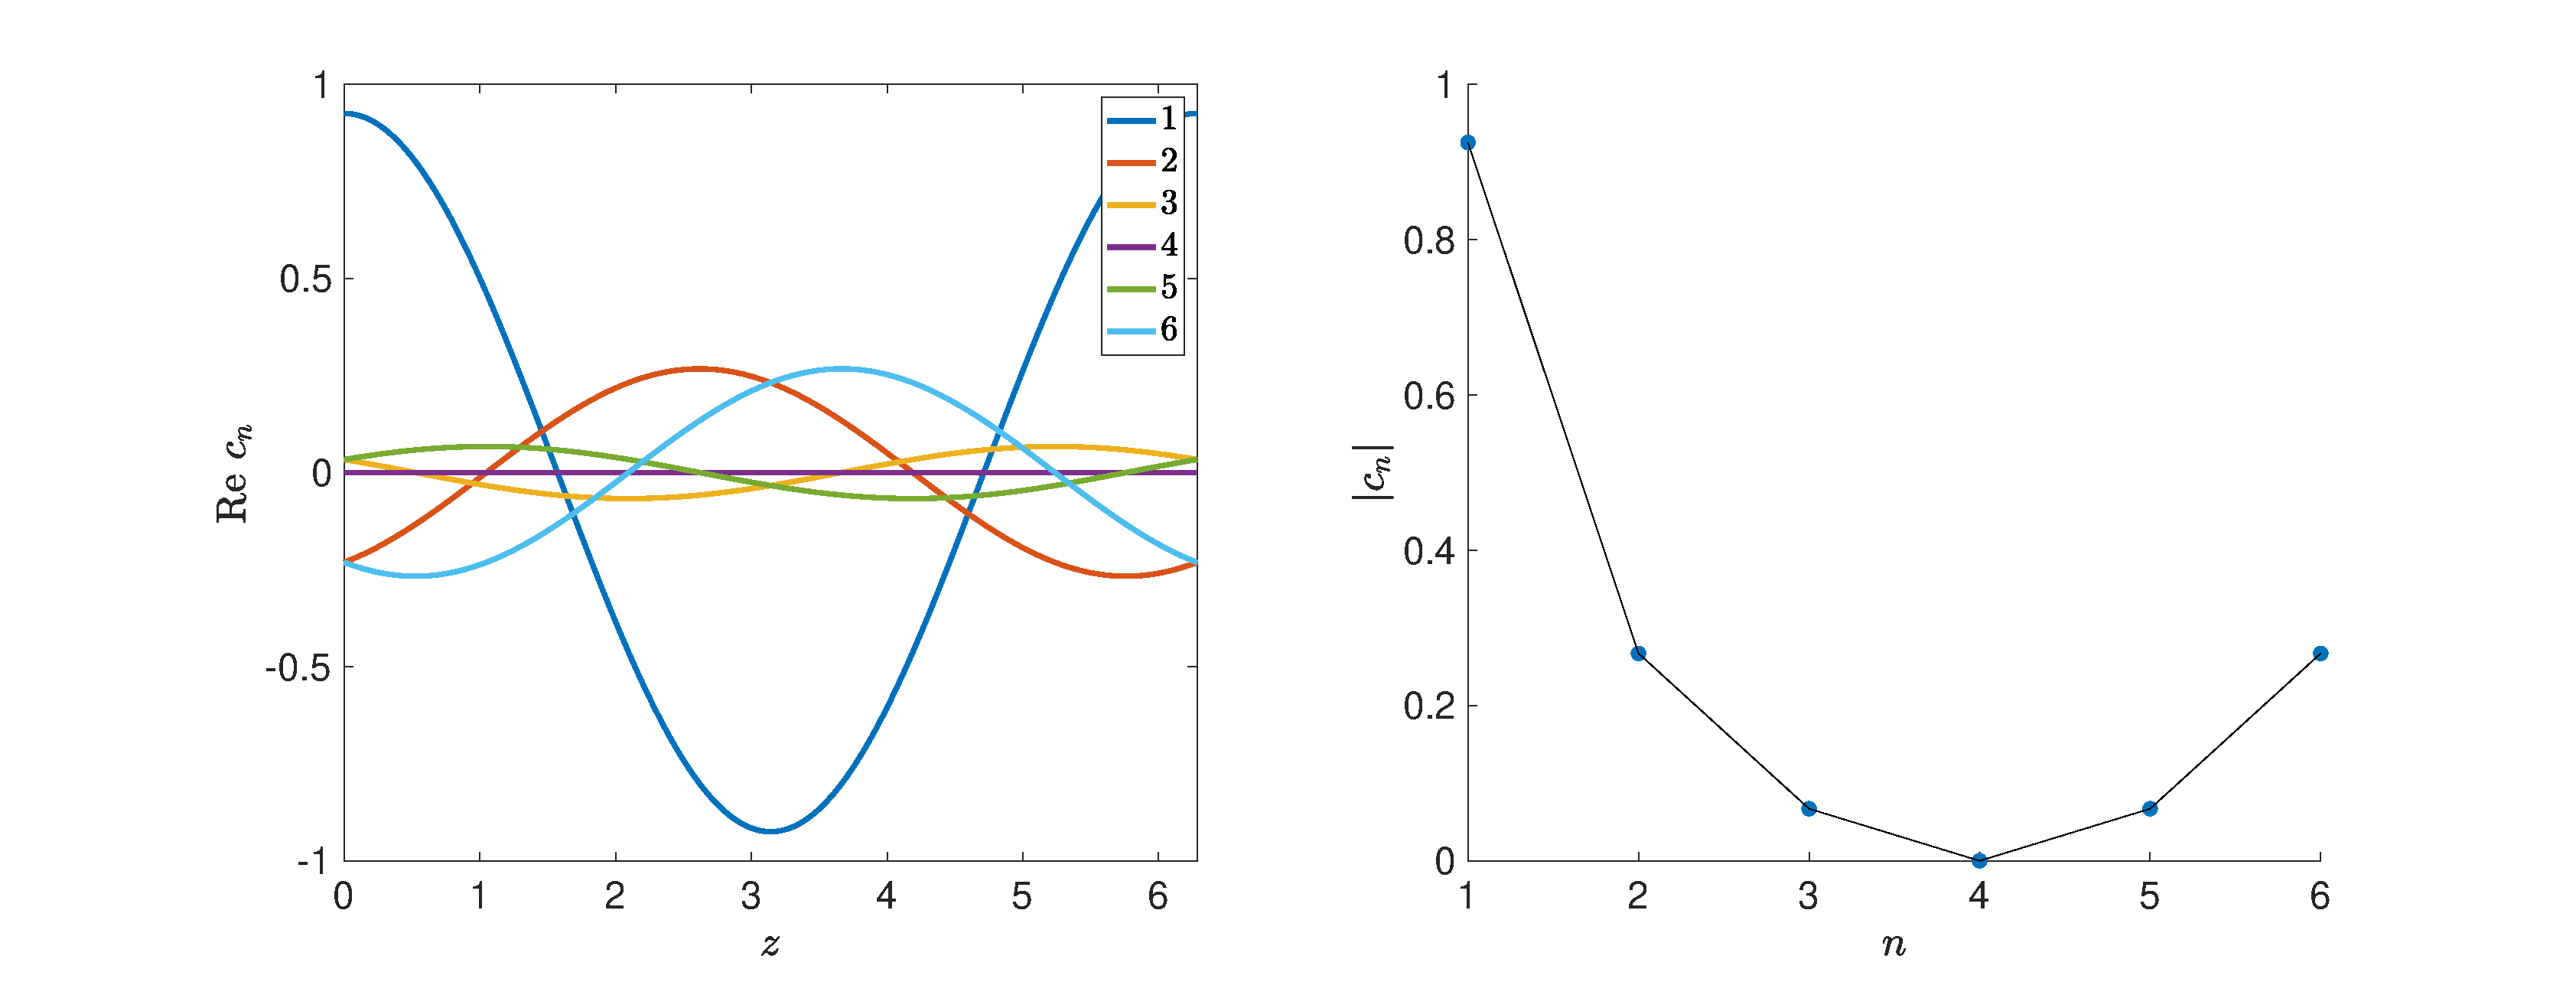
\includegraphics[width=14cm]{images/evenhole6}
\end{tabular}
\end{center}
\caption{Standing wave solution $c_n$ for twisted multi-core fiber with $N = 6$ and $\phi = \pi/6$. Time evolution (left) and magnitude of solution at lattice points (right). Node 1 has maximum intensity, and opposite node 4 has zero intensity.}
\label{fig:twistcn}
\end{figure}
Future research involves more complicated arrangements of fiber bundles, such as concentric rings, a Lieb lattice, or a honeycomb lattice \cite{Lumer2013,Marzuola2019}. For some of these geometries, localized breather solutions have been found, for which the bulk of the energy is confined to a small number of lattice points, but no systematic study of their existence and stability has been done to date.

\bibliographystyle{amsplain}
\footnotesize{ \bibliography{researchstatement.bib} }

\end{document}
